\documentclass[uplatex]{suribt}
%\documentclass[oneside]{suribt}% 本文が * ページ以下のときに (掲示に注意)
\title{超音波計測による深層学習を用いた菅内流体の気相体積率推定}
%\titlewidth{}% タイトル幅 (指定するときは単位つきで)
%\centering
\author{松原貞徳}
\studentid{37246227}
%\eauthor{Sadanori Matsubara}% Copyright 表示で使われる

\supervisor{高木周教授}% 1 つ引数をとる (役職まで含めて書く)
%\supervisor{指導教員名 役職 \and 指導教員名 役職}% 複数教員の場合,\and でつなげる
\handin{2026}{1}% 提出月. 2 つ (年, 月) 引数をとる
%\keywords{キーワード1, キーワード2} % 概要の下に表示される
\usepackage{float}
\usepackage{amsmath} 
\usepackage[dvipdfmx] {graphicx}
\usepackage{amsfonts}
\usepackage{comment}
\usepackage{geometry}
\usepackage{bm}
% \usepackage{bbm}
\usepackage{subcaption}
\usepackage{url}
\newtheorem{lemma}{補題}[section]
\makeatletter
  % subsectionの下マージンを小さく
  \renewcommand{\subsection}{%
    \@startsection{subsection}{1}{\z@}%
    {0.4\Cvs}{0.1\Cvs}%
    {\normalfont\normalsize\headfont\raggedright}}
\makeatother
\begin{document}
%\Studentid{37246227}
\setcounter{tocdepth}{2}%\subsectionが目次に含まれるようにしている
% \begin{center}
% \Large{超音波計測による深層学習を用いた菅内流体の気相体積率推定}\\
% \normalsize{松原貞徳 指導教員 高木周教授}\\
% \normalsize{void fraction prediction from ultrasonic measurement technique using deep learning}
% \end{center}
\maketitle
\tableofcontents
\chapter{序論}
\section{研究概要}
数々の調査により、海底には豊富な海底資源が存在することが知られている。日本近海の海底資源を掘削、開発する研究は長年続けられてきたが、経済的な理由で実用に足る運搬手法は開発されていなかった。しかし近年では、メンテナンスが容易かつ運搬の仕組みが簡素であるとの理由でエアリフトポンプという機構が注目を集めている。この手法は海底に管をたてかけて、管内下部に資源と海水の混合流を流し込み、それらに圧縮空気を注入し空気が混合流と共に上昇しようとする力を利用して運搬を行うというものである。
当該手法の技術的課題としては、注入する空気の量を極めて厳密に制御する必要があるというものが挙げられる。空気が少なすぎれば運搬を行う能力が不足する一方で、注入量が多すぎれば流動の様式は環状流に推移し、大きく運搬性能が低下するという性質がある。効率的な運搬のためにはこれらの注入量を適切に制御する必要があり、管内の気相体積率を測定し制御の情報として利用しようとする案がある。しかし、そのような技術は現在開発されていない。運搬する流体は不透明流体であるとの理由から、従来支配的であった光やγ線を利用する方法は使用できない。また、鉱石を運搬する都合上、管にプローブを挿入するような侵襲的な計測手法は好まれない。\par
そこで注目されているのが超音波計測である。超音波はその反射波を測定し情報を利用することで不透明流体に対しても測定が行えると期待されており、また、流れに対して与える影響も無視できるほどに微弱である。海洋技術研究所で行われた実験データの提供を受け、計測された信号波形データと相体積率の間の関係性を解明し新たな計測技術の開発を行うことが期待されており、本研究室ではその協力を受けて技術開発を行った。
\section{研究の背景}
エアリフトポンプを用い海底資源を揚降するプロジェクトが進行中であり、本研究室では開発の前段階としての性能評価の正当性を検証するため超音波計測による物理量の測定技術の開発が期待されている。より詳しく言えば、実海域において最適な管径や空気吹き込み条件を取得できればシステム設計にとって非常に望ましく、そのための構成方程式の精度検証により実測値を必要としている。
\subsection{エアリフトポンプを用いた揚降実験に関する研究}
\subsection{混相流の力学に関する研究}
\subsection{混相流計測手法に関する研究}

エアリフト揚降システムを開発する上で、入念な技術調査が行われてきた。流体力学においてはその計測手法が長らく研究されてきており、理論的工学的研究が数多く存在する。その中で、下にあるようないくつかの技術が検討された背景がある。\par
・写真計測\par
・締め切り法\par
・PIV,PTV\par
・電気プローブ、光ファイバプローブ、ワイヤメッシュなど\par
・X線・γ線\par
・静電容量方式\par
これらのうち、実験により写真計測、PIVなどの手法がまず検討されてきた。しかし、撮影された画像から有益な情報を得ることは困難であった。\par
次に、電気プローブ、光ファイバープローブ、ワイヤメッシュなどの方法が検討されてきた。しかし、これらは粗大固体粒子を含む系には適用不可という側面がある。\par
X線・γ線を利用する方法に関しては、固気液三相(三成分)だと体積率を取得する技術が存在しないことに加え、放射線を取り扱うので大口径化などの点で見通しが不透明であるという問題点があり、静電容量方式でも固気液三相だと体積率を得られず、軸対称性が崩れた場合などは計測できないことが予想されるのである。これらの理由により、超音波によって流体を計測する試みが行われてきた。様々な取り組みが各所で進行中であるが、例えば共同研究を行っている北海道大学においては純粋な物理学的アプローチに基づく技術開発が行われてきた。しかし、混相流には膨大な変数が存在しモデル化が極めて困難である。従来支配的であった光学的な計測も使用できず、また、光学的計測と異なり超音波計測においてはノイズの影響が極めて大きいことが実験的に知られており、信号波形から人為的に特徴を抽出するアプローチが限界に達しつつある。\par
本研究室においても諸先輩方によって研究がなされてきている。そのうち近年のものを簡単に紹介する。\par
例えば2023年には、管の断面を模した系での数値計算および、得られた信号波形をもとに気泡のサイズと位置を機械学習によって推定する研究がWangによって行われた。この中で、気泡がたった5つかつシミュレーションという条件下でも予測が困難であると指摘されている。しかし、データセットの統計に関する議論が行われていない。よりバランスされたデータを用いることによって再現できる可能性がある。また、その中で実機実験の必要性と3次元シミュレーション、固気液三相流のシミュレーションを行うことを提案している。\par
2024年には尾花によって上昇気液二層流の超音波計測の技術がまとめられ、超音波のTime-stripイメージをもとに学習させるアプローチにおいてスラグ流・チャーン流の識別が行われた。また、この中で数値計算による計測データを学習させることが提案されている。\par
2025年には渡辺によってCNNを用いた相体積率及び見かけ流速の推定が行われ、有効な前処理手法についての調査が行われた。その中で二相流においては高精度での推定が可能だが、固気液三相流では困難であると主張した。しかし、全体的にデータが極めて少なく、それゆえ十分なテストデータを用意できず、有効かどうかの検証が十分ではない。また、学習されたパターンの物理現象を、計算機理論と照らし合わせて議論する必要がある。

\section{研究の目的}
以上に述べたとおり、従来の流体計測技術では当面の技術的課題を解決できず、我が国においては主に北海道大学と我々のチームで超音波での技術的開発が目指されてきた背景があり、本研究室においても技術的困難さが確認されている。前述のとおり系が極めて複雑であり、物理的な現象論的アプローチも限界に達しつつある。そこで、本研究においては複雑系の取り扱いに強みを持ち、それらの特徴、表現をデータから取得できる可能性のある深層学習の技術を用い技術的課題の解決を目的とした。とくに、相体積率を推定する目的のもと実験データおよび数値計算を活用してデータを入手し、現象論に基づいた考察を行うこととする。
\section{本論文の構成}
まず初めに研究の発端となった状況及びその動機に触れることによって動機を示し、そのうえで各所で様々な研究が行われてきたことを述べた。その中で顕著なものに焦点を当て、流体工学分野での混相流分野の概要や、流体計測技術を調査した。それを受けて、本稿において数値計算を活用して得られた知見やデータを信号処理によって適切に機械学習・深層学習と組み合わせ、目的の達成を図った記録を示す。その際、使用した技術を各分野ごとに分けて可能な限り綿密に記した。本稿の核をなす数値計算、そのデータの処理を体系づける信号処理、そして得られたデータをもとに予測を行う深層学習について概論を示し、それらに基づいて本稿における数値計算の結果とそれに基づく知見、さらにそのデータを学習させた場合の性能と評価、今後の展望を示す。
\chapter{混相流超音波計測}\label{experimental settings}
超音波とは振動である。それゆえ、媒体を必要とする。その媒体の物性によって減衰や反射の特性が変化するが、伝播した超音波、すなわち計測物体の振動の情報を圧電効果を利用することによって電気信号の形として取得し、適切に変換することによってはじめて信号波形を計測することが可能となる。それら信号は電磁気学的に設計された電子回路によって適切に処理され、信号波形として対象物を計測した際の情報を利用できる。本研究においては電気回路については簡単に触れるのにとどめることとし、あくまで取得された計測波形に基づいて議論を行う。\par
ところで、音波信号波形の解析の研究分野では、例えば人間の音声を計測・解析し音声を認識するシステムを構築する研究が盛んにおこなわれており、機械学習のような統計的なモデル化の技術と密接に関連している。そういった音声の計測波形のスペクトログラムには多くの要素が観測されるが、本研究分野においてはそれほど多くの要素は存在しない。今回は物理量を測定する目的ゆえ一つの周波数帯のみの超音波を利用しているからである。単一の周波数を用いればフーリエ解析を行った際にスペクトルの解釈が容易となり、要因の特定に寄与する。さらに、今回はその対象も混相流というやや特殊な系である。先行研究の調査の際、音波の信号処理と機械学習に基づいた技術は高確率で言語処理と結びついているが、今回のような特殊な系でも有効かどうかの判別には注意が必要である。\par
以下、混相流の超音波計測について記す。混相流、例えば気液二相に関しては画像解析に基づくいくつもの手法が存在しており、例えば坂口ら\cite{sakaguchibubble}の研究によれば、えは、周波数、強度、波形で表すことが可能である。すなわち$A$を振幅、$\omega$を各振動数、$\phi_0$を位相とした際に、音は 
\section{計測機器(実験系)}
協力を受けた海洋技術安全研究所の実験設備を以下に示す。
産業技術総合研究所の実験設備の写真を以下に示す。これに関しては、超音波計測が不十分であったため解析も検証も行っていないが、大まかなイメージを掴むために掲載することにする。
これら実験系は、上昇鉛直管における固液二層流、気液二層流、固気液三相流を超音波で計測した場合の信号データのほか、空間平均の相体積率や画像データに関しても取得できることが目的とされており、いくつかの設備が複合されてある。信号データを取得する目的でトランスデューサが、画像データを取得する目的で超音波照射と同期する設定のもとハイスピードカメラが設置されている。なお、空間平均の相体積率は締め切り法と呼ばれる手法で計測されており、これは上下バルブを同時に遮蔽し、バルブ間に取り残される媒体を測定する手法である。固相に関してはガラスビーズの個数が数えられ、気相、液相に関しては液相のみ体積率の比として測定される。1から液相、固相の割合を引くことによって気相の体積率が求められる。
概念図を以下に示す。この図のポンプにより流体の駆動力を得、適切に空気を注入することによって混相流が再現される。
\section{計測原理}
\subsection{サンプリング定理}
連続時間と離散時間の間の穴埋めを行う。ある条件を満たした場合、離散的な信号から連続信号を復元できるが、その条件について解説したものである。sinc関数との畳み込みにより実現可能であり、そのための条件について示す。
\subsection{離散化}
いくつかの信号処理を行う場合、信号系列に対してフーリエ変換を行う必要がある。しかし、信号は計算機においては離散的であり、それらに対応する必要がある。
定義域が有限であること故にいくつかの対応が必要である。例えば、
\begin{equation}
    x[n+mN]=\frac{1}{N}\sum_k^{N-1}X[k]exp(j\frac{2\pi kj(n+mN)}{N})=\frac{1}{N}\sum_k^{N-1}X[k]exp(j\frac{2\pi kjn}{N})exp(2\pi kjmN)
\end{equation}
のように、周期的に拡張されてしまっている。
そこで、離れれるほど減衰する重みを付ける。これがHanning窓とよばれ、中心をピークに
\subsection{フーリエ変換の派生}
時間波形に対し、定常の仮定を置くことができるかは定かではない。そこで、短時間においては定常であると考え、その信号に対して適切な窓をかけてフーリエ変換を行う。これを短時間フーリエ変換と呼び、それらによって変換されたものは、強度と時刻周波数の情報をもつと考えられ、これがスペクトラムと呼ばれる。
\section{超音波画像法}\label{ultraimage}
超音波画像は、特に医療分野で広く用いられている。妊婦のお腹の中の胎児を可視化しようとした場合には、人体に影響を及ぼす電磁波などよりも、力学的な刺激であり人体に無害な超音波を用いて可視化することが好まれる。ここで用いられているのが、超音波画像法と呼ばれる方法である。これは、超音波パルスを照射してその透過波、反射波を記録し、その強度に応じて色分けして表示することによって画像を得る手法である。これらは、一般に信号波形の包絡線を取得し、適切に対数圧縮を施すことによって実現される。
\section{ノイズ除去}
本研究における学習データに関してだが、計測機器の不具合といった何らかのエラーにより不適切な値を取ることがある。そういった値は適切な学習を阻害しうるので適切に除去する必要がある。これらに関してはデータ分布を適切な手法で確率分布としてモデル化し、値を取る確率が極めて小さいものを外れ値として除外するという案が考えられる。\par
今回、実機データとその際の測定記録を拝見した際には、恐縮ながら命名が誤っていたり、データが破損している事例がしばしば見られた。例えば、実機測定データは存在するがそれらに対応する相体積率の目標値がなかったり、その逆がみられた。これらは筆者が手作業で確認し、修正した。今後このデータに基づいて解析を行う場合には、解析の担当者の負担が増すことがあるので、注意されたい。\par
また、後述するように、実機データにおいてはシミュレーションと異なり尖ったピークは一般に現れない。実際には尖った先端を切り取って台形にしたような信号波形になることが確認されている。これらに対し、適宜関数をフィッティングしてピークを補完し、より正しい値でのスケーリングを行うことが考えられる。その技術は、例えば\cite{kyodaisenpai}の技術を使えば解決できる可能性はある。
\chapter{数値計算}
本研究においては、実機計測データに加え、シミュレーションによって生成した計測データも利用した。すなわち、シミュレーション生成のデータをもとに機械学習モデルを訓練・検証した後に実機データにおいてそれを評価するモデルも存在する。実機を模した機械学習用データを作成することを目的とした。
\section{超音波の性質}
音は、周波数、強度、波形で表すことが可能である。すなわち$A$を振幅、$\omega$を各振動数、$\phi_0$を位相とした際に、音は 
\begin{equation}
    f(t)=Asin(\omega t +\phi_0)
\end{equation}
として表現されるので、周波数$f=\omega /2\pi$, 強度$I=2\pi Z_0 A^2f^2$, 波形$s$
として表現できる。  
超音波の性質として、周波数が高いほどまっすぐ進みやすい一方で、強度が減衰しやすいというものがある。超音波は物質の界面で反射する性質がある。これらの反射と入射・および減衰と透過の影響を特徴づける量が音響インピーダンス$Z$である。一般に知られている物性値として以下のものがある。

$Z_0$が大きく異なる物質の界面では超音波は反射する。ゆえに超音波は液相から固相に入ることはできるが、気相に衝突した際にはほぼ全反射される。これらは実験的にも観察されている。
ゆえに、気液界面での超音波の反射を計測することによって鉛直管内流の気液界面を取得できる。

\section{計算原理}
本節ではkwaveの動作原理を簡潔に記すことを目的とする。詳細は参考文献\cite{treeby2010k}を参照されたい。\par
超音波の伝播については波動方程式によってモデル化されており、系の時間発展を記述することが可能である。この方程式は原理的には二階の非線形偏微分方程式であるが、流体の保存則を活用することによって複数の一階偏微分方程式に分解することができ、数値的にも安定した計算が可能になる。
例えば、減衰なしの流体のもっとも単純な系の運動を記述する方程式として運動量保存則、質量保存則、圧力ー密度の関係式が存在する。これらはそれぞれ
\begin{align}
    \frac{\partial \mathbb{u}}{\partial t }= -\frac{1}{\rho_0} \nabla p \\
    \frac{\partial \rho}{\partial t} = - \rho_0 \nabla \cdot \mathbb{u} \\
    p= c_0 ^2 \rho
\end{align}
が挙げられるが、これらを整理すると
\begin{equation}
    \nabla^2p - \frac{1}{c_0^2} \frac{\partial ^2 p}{\partial t^2} =0 
\end{equation}
の、波動方程式を得る。\par
すなわち、これらの波動方程式の解は、流体の保存則の解と等価である。
実際は減衰などのより現実に即した効果を付した項が追加され、より複雑な方程式となる。これらの式を離散化することによって、連続な量を対象とする本来の偏微分方程式を計算機で数値的に解くことが可能となる。
\subsection{疑似スペクトル法(pseudospectral method)}
シミュレーションにおいてはいくつかの数値的なモデルが存在する。そして、それらへの最適なアプローチは系に依存する。それらに対して、heterogeneous(不均質)な系、つまり様々な材質から成る系についての解を求めたいとする。こういった問題を解くには、有限差分法(finite difference)あるいは有限要素法(finite element)が考えられるが、有用な精度を達成するには音波長あたり10点が必要である。\cite{treeby2010k}これらの方法では、一般的なコンピュータでは対処不可能であったりする。$3 \ \mathrm{MHz}$の超音波を使い、$150 \ \mathrm{mm}$の系を再現しようとした場合には、倍音(second harmonic)を含めて600波長をとる必要があり、その方向だけでも$6 \times 10^4$のグリッドを取る必要がある。3次元で行う場合には総数は$10^11$を超え、数百GBのメモリが必要になる。時間幅についても、シミュレーションの安定性を担保するためにもより小さく幅をとる必要もあるので、シミュレーションはさらに困難になる。\par
これらは、有限差分法が、もとの関数の近傍でとくことに起因する。勾配を評価する際、高精度の値を得るにはより高次の多項式をフィッティングする必要があるのがその所以である。高精度を得るためにより多くのグリッドを得て、かつより高次の関数を必要とする。これらに対処するのがフーリエスペクトル法である。この手法は、データ点すべてにフーリエ級数を割り当てる。基底関数が正弦波的な形状を持つために、有限差分法と異なり高次の多項式を必要とせず、かつ2点でフィッティングできるので必要なグリッド数も少ないのである。よって、波動伝播においてはより効率的な計算手法であるとされる。
\subsection{安定性解析}
系の方程式を記述して、それを数値的に解く場合にはいくつかの検定が存在する。
\begin{description}
    \item[1.]離散化に伴う連続量との乖離
    \item[2.]安定性解析
    \item[3.]計算結果の正しさ
\end{description}
離散化に関する議論はkwaveのマニュアルにおいて詳細になされており、ここでは割愛する。よってここでは、解の安定性について述べる。\par
離散化に伴う量は、$\Delta t $を十分小さくとることによって導関数に一致することは議論によって示された。よって、ここで重要なのは数値的な誤差が時間発展によって増大してしまうか否かである。これらは、十分$\Delta t $を小さくとることが望ましい一方で、計算時間の制約からできる限り粗くとることが望ましい。しかし、ここでもいくつかの検定が存在する。ただし、一般に適切な領域で$\Delta t $を小さくとって計算をやり直し、その値が収束することによって正しさを証明する手法である。低周波の波長の伝播の計算はより高周波の伝播によって保障されているので、高周波の計算がそれを担保するのである。しかし、データセット一つ一つにその検定を行うことは、今回の目的上難しい。よって、適切な理論解析によってその計算の正しさを保障するのが望ましい。

\section{計算系の設計}
数値計算を実行するためのオブジェクトを点群として定義し、それらに対し適切な物性値や信号遅延などを与えることによって実機に近い測定データを得ることが可能となる。計算系において存在する媒質は、固気液三相流の場合も含め石、塩化ビニル、水、空気、ガラスであり、これらをトランスデューサによって計測するという設定をなす。一般的な設定において、2次元では任意のセンサー配置ができる一方、現実の測定に即したビーム収束などは再現できない。一方、3次元では送信器、受信器でそれぞれ一つのトランスデューサしか実装できないが、各素子への信号の送信に時間遅れを持たせて、超音波に指向性を持たせることが可能となる。計算に使用した各種物理量はconfig.jsonにも記載されているので、そちらを参照されたい。以下は、それぞれの設定理由を示す。
\subsection{物性値}
物性値に関しては、現在に至るまでの数々の実験から再現可能な量が測定されてある。まず初めに、計算系において物性値を以下のように設定した。
\begin{table}[]
    \centering
    \begin{tabular}{c|c|c|c}
    \hline
         substance & Acoustic impedance & density & sound velocity \\
         \hline
         air&  0.00043 & 1.3 & 330\\
         water& 1.5 & 1000 & 1500\\
         glass & 18.9 & 2200 & 5300\\
         \hline
    \end{tabular}
    \caption{acoustic impedance used in the experiment}
    \label{tab:acoustic impedance}
\end{table}
これらに基づき、超音波伝播が数値的に計算され時間発展が表現される。
\subsection{グリッドサイズ}
次に、計算を行う上では格子点、その幅を計算機の性能を鑑みながら決定しなければならない。理想的には、計算機の性能が、シミュレーションに必要な性能を大幅に上回っている状態が望ましく、計算機の制約を考えずに設計したい。しかし、研究室の計算環境ではやはりそれも考慮して計算系の設計をする必要があった。以下、計算系の要件を示す。\par
まず実験設備のスケールとしては、トランスデューサが超音波を照射しその反射波を記録する目的から、
\begin{equation}
    l_x\ [\mathrm{mm}] > 82 \ \mathrm{mm}
\end{equation}\par
である必要がある。また、幅に関しては管の直径よりも太くある必要があるので、
\begin{equation}
    l_y \ [\mathrm{mm}]> 32 \ [\mathrm{mm}]
\end{equation}
が必要である。
なおこれらは下限であり、実際はもう少しゆとりを持たせることが好まれる。\par
他方、計算を正確に行うための計算理論による要件を示す。まず初めに、今回は波動伝播をシミュレートするので、波動が次のグリッドに伝播する前に時間更新を行うことはできない。また、その波動の位相も正確に取得せねばならない。ゆえに、$\lambda_{min}=c_{min}/f$,$c_{min}$を、系の構成要素の中での最も遅い伝播距離として
\begin{equation}
    2 \Delta x\ [\mathrm{m}] < \lambda _{min}\ [\mathrm{m}]
\end{equation}
である必要がある。\cite{treeby2010k}
例えば固液二層の場合では律速が水なので$c_{min}=1500 \ [\mathrm{m/s}]$, 気液・固気液では空気が律速となるので$c_{min}=340 m/s$となる。
ゆえに、例えば固液を例にとると、現在使用している超音波の波長が$4 \ \mathrm{MHz}$であるので
\begin{equation}
    \Delta x \ [\mathrm{m}]< \frac{1500}{2 \cdot 4 \cdot 10^6} \ [\mathrm{m}]= 0.1875 \ [\mathrm{mm}]
\end{equation}
を満たさなくてはならない。ただし、2倍、3倍などの高周波成分などの量を再現しようとした場合には、その分だけ小さくとる必要がある。これらは、フーリエ変換のスペクトルで$12 \ [\mathrm{MHz}]$のピークがわずかに見られたためそれらを再現する目的で$0.0625 \ [\mathrm{mm}]$よりも小さい値に設定する必要があった。\par
ここで、格子点数の要件について記す。今$l_x =N_x \cdot dx > 82 \ \mathrm{mm}$であるので、
\begin{equation}
    N_x > 1312
\end{equation}
が示される。計算機上は2の累乗だと計算効率が良いので、$N_x=2048$を採用してある。
同様の議論で$N_y > 512$が必要だが、これでは計算系の境界に接してしまうので望ましくない。そこで、それよりも大きくかつ効率が良い値として$N_y=768$を採用した。\par
最後に、$N_z, dz$について触れる。これらは、計算機の上限から$N_z=128$とした。これらによりGPU上で20GBの仮想メモリが割り当てられ計算が実行された。
\subsection{固液二層流}
系を規定する媒体は、ガラスおよび水の二種類である。また、実験記録にはガラスビーズの直径が2.5 mmと記載されてある。よって、事前にガラスビーズの個数を規定しておき、それを空間的に配置して計算系を作成した。この際、複数のガラスビーズの座標はBox-Mullar法と呼ばれる乱数生成のアルゴリズムをベースに、適当な検定を設けることによって生成した。以下にその詳細を示す。これらによって生成した座標は$\{x | x\in[-1,1]\},\{y | y\in [-1,1]\},\{z |z \in [0,1]\}$ の区間で生成されており、これをグリッドサイズの分だけ拡大することによって計算系の座標として利用してある。
トランスデューサの設定としては以下のものを用いた。


\subsection{気液二層流}
今回は空気と水の二種類によって系が決定される。固液二層との違いは、気泡の形が球形を成すとは限らず、またその形状も複雑であり、体積も一定でないということである。著しく非軸対称であり、分裂の最中のもの、合体の最中のものなど混迷を極める。一方で、気液二相に関しては画像解析に基づくいくつかの知見が存在しているのも事実である。例えば坂口ら\cite{sakaguchibubble}の研究によれば、大きい気泡は菅中央に、小さい気泡が間壁付近に分布することが明らかになった。また、古典的な教科書である\cite{batchelor2000introduction}によれば、$6\times 10^{-4}c.c$程度の小さい気泡に関してはほぼ球であると仮定してよく、この値を超えると扁平となり振動しながら上昇する。次に、体積が5ccよりも大きくなると球の一部を切り取ったような形になり、また、その仰角は泡の体積によらず46°~64°となる。最後に、菅いっぱいを占めるような大きな泡に関しては、形状定数$\alpha$、気泡の上昇速度$U$,重力加速度$g$、よどみ点における気泡表面の曲率半径$R$を用いて
\begin{equation}
    \alpha^2 U^2 = gR
\end{equation}
の形状をなす。また、$U$は円管の内径を$D$として$0.48\sqrt{gD/2}$に等しく、$R/D>0.26$ならば半径$R$の帽子型形状の泡よりも小さい。ゆえに、管を埋めるほど大きくない泡は大きい泡へと追いついて合体することを示すという。最後に、これら帽子型から十分下方では、質量保存の式から
\begin{equation}
    \pi \frac{D^2}{4} U=\pi {\frac{D^2}{4} - (\frac{D}{2}-d)^2}\sqrt{2gx}
\end{equation}が得られ、基本の先端からの距離を$x$として
\begin{equation}
    \frac{2d}{D} =1 -\sqrt{1-\frac{U}{\sqrt{2gx}}}
\end{equation}
の関係式を成すという。さらに、村井の研究\cite{村井祐一20222022.T011}らにより気泡径とその分布が統計されており、その形状は、ポアソン分布に酷似している。
これらから、技術的に大まかにモデル化可能な領域と、その正しさが確認される。すなわち、超音波伝播をシミュレートする上で気泡の数$N$、形状の関数$S_i$、気泡それぞれの座標$\mathbf{r}_i$を決定する必要がある。ここで、形状のモデル化に関しては極めて難しいので、構成要素としては球あるいは円柱を組み合わせただけとする著しい簡略化を行った。ゆえに、これら形状は球の直径$D_i$と円柱の高さ$h_i$の関数としてよく、また、座標$\mathbf{r}_i$の確率分布は$D_i$によって規定されると仮定できる。
これらから、暫定的に条件を満たす分布を以下のように定義して以下議論を進めることとする。$N$は既知とする。

\begin{align}
    &D \sim Pr(\nu) \\
    &h \sim Uni[0,a] \\
    &S =\left\{ \,
    \begin{aligned}
        &Sphere  (0 < D < 1 mm) \\
        &Oblete (1< D <10 mm)\\
        &Spherical-cap (10mm< D )\\
        &fill-bubble 
    \end{aligned}
\right.
\end{align}\par
ここで、spherical -capに関しては仰角が46~64°と定まっているため、60°と定義することによって、曲率半径の関数として体積を導出できる。高校レベルの数学でこれは計算可能で、$\theta=\pi/3$の時は
\begin{equation}
    V(R)=\frac{16-9\sqrt{3}}{24}\pi R^3\sim0.0539R^3
\end{equation}
と計算できる。これらを実装することにより、上昇気液二層流における気泡流、スラグ流、チャーン流、環状流のうち気泡流と環状流のシミュレーションを行えることが期待される。スラグ流・チャーン流は著しく不規則なので、大変な技術的困難が予想される。


\chapter{機械学習}
機械学習は、データからパターンを抽出する技術である。より詳しく言えば、入力と出力の関係をモデル化し、モデルによる予測結果と目標値との誤差が小さくなるようにモデルのパラメータを更新する技術である。このような更新を行うためには誤差関数の値を最も小さくする方向に適切にパラメータの更新量を求める必要があり、そのために誤差関数そのもののパラメータに関する勾配を評価する必要がある。パラメータの更新量を求める最適化アルゴリズムには、確率的勾配降下法(Stochastic Gradient Decent,SGD)に基づいた数々の手法が存在する。これらについて詳細はBishop\cite{Bishop:DeepLearning24}に譲るが、本稿においては核となる部分に焦点を当て、網羅的に記述することとする。

\section{要素技術}
\subsection{分類と回帰}
近年の深層学習では生成モデル(generative models)の応用が盛んである。自然言語やロボットの動作命令を生成する技術開発が盛んであり、今日のAIブームといえばそれらを指すことが多い。しかしそれらを行うには、入力と出力の関係を確率的にモデル化し、それらからのサンプリングとして利用する必要がある。そのモデル化に用いられるのが機械学習である。より厳密にいえば、$D$次元の入力$\mathbf{x}$から目標となる$t$、ひいてはそれらへの関数を発見することを目的とする。ここで、$t$に関しては連続かどうかの場合分けがなされる。今回のような相体積率を予測する場合には連続な値を取る回帰モデルを、流動様式を予測する場合にはそのカテゴリを離散的な値で出力する分類モデルを訓練することが求められる。\par
つまり、回帰の場合には予測分布$p(t | \mathbf{x},D)$を求め、確率分布に応じて期待値を評価するという手続きを経るのに対し、分類の場合にはある入力がそのカテゴリに属する確率$p(C_k | \mathbf{x},D)$を求め、それぞれのクラスに属する確率を計算した後に最も大きな確率を持つカテゴリへと分類するという操作が行われる。ほかの例をあげると、化学プラントにおける生成量や株価、住宅価格のような連続な値を取る場合は回帰タスク、ある画像が犬か猫かを判別するような、離散的な値を予測したい場合は分類タスクだと理解される。\par
本稿においてはモデルと呼ぶ場合には、ニュートン力学のような決定的かつ実存的な物理モデルではなく、確率・統計的な文脈で入力と出力の間の関係を規定するものという意味合いで使用している。それゆえ、各種確率モデルに含まれる数々のパラメータに本質的な意味を持つことはなく、あくまでデータセット依存のものであることに注意されたい。\par
また、本稿では機械学習の中でもニューラルネットベースの手法に注目して調査を行った。機械学習の手法には、統計・関数解析の分野で発展したSVMやカーネル法のような手法もあれば、線形分類器の重ね合わせと多数決によって予測を行う決定木、そして深層学習に代表されるニューラルネットベースの手法がある。本稿は、ニューラルネットベースでの手法、すなわち深層学習に着目し超音波データから流動様式や相体積率のような値を予測する試みで研究を行ったものである。
\subsection{誤差関数の勾配の評価}
先に、機械学習における学習とは、目標変数の値と予測値との誤差、あるいはそれらが引き起こす損失を小さくするようにモデルのパラメータを更新すると述べた。つまり、誤差関数をモデルのパラメータに関して微分し、その導関数の値に応じてモデルのパラメータの変化量を求めるという手続きを必要とする。ただし、その誤差関数の微分を評価する手法に関し、関数が高度に非線形かつ、閉じた形での関数が求まらない場合が数多く存在する。それらへの解決策として、ある関数を特定の変数で微分した関数を出力する技術が自動微分と呼ばれ、誤差逆伝播の基礎をなす。
誤差逆伝播とは、簡潔に言えば出力層における出力値と目標値の誤差をもとに最終層のパラメータに関する誤差関数の勾配を求め、それを再帰的に行うことによって全ネットワークにおけるパラメータの勾配を入力側にもどって計算していくというものである。ネットワークのある層におけるパラメータを計算したい場合、それらすべてと前のノードの入力の線形和および
\subsection{正規化・正則化}
今回設計したモデルには、学習を円滑に行うためにいくつかの統計処理を施してある。今回、シミュレーションで得られるデータは数khPaにも及ぶ圧力変動であるのに対し実機試験で得られるデータはトランスデューサの―2~+2Vの範囲の電圧変化である。シミュレーションのデータを学習に利用し、実機データでの性能をテストするというアプローチをとるとは言え、そのままでは入力データにおける数値的な変動があまりに大きい。ゆえに、データのスケールをそろえるという操作が重要となる。このような操作は正規化と呼ばれ、単にシミュレーションと実機に見られる値の差異のみならず、同じ入力間のデータや、隠れ相を通った後のデータに対しても同様に重要である。使用した正規化のテクニックは以下である。\par
・データ正規化\par
・バッチ正規化\par
・レイヤー正規化\par
これらはやや区別が煩わしいので、以下に詳細を追記する。
バッチ正規化\par
これらは、バッチサイズ$K$に対し
\begin{align}
    \mu_i& =\frac{1}{K}\sum_{n=1}^{K}a_{ni}\\
    \sigma_i^2& =\frac{1}{K}\sum_{n=1}^{K}(a_{ni}-\mu_i)^2\\
    \hat{a}_{ni}&=\frac{a_{ni}-\mu_i}{\sqrt{\sigma^2+\delta}}
\end{align}
の定義の元で
\begin{equation}
    \tilde a_{ni} = \gamma_i \hat{a}_{ni}+\beta_i
\end{equation}
の操作を施す。
つまり、活性化を行う前の値を、バッチサイズで平均0、分散1の数の集まりに計算しなおし、さらに適切な値でその操作の埋め合わせを行う。ここで、δは数値的な不安定性を防ぐためのものである。
これらはモデルを設計する際に、畳み込みの層と層の間に行われるような形で定義され、モデルのパラメータの一部として訓練の際同時に求められる。\par
ここで、訓練の際はいくつかのデータをひとまとまりに(=バッチ)して学習させたが、新しいデータでの予測を見たい場合には、入力データは一つしかない。もう一度訓練用データを用いて全部計算すればそのようなパラメータは得られるが、計算コストが高いため移動平均の量を用いる。つまり、訓練時に
\begin{align}
    \bar \mu_i^{\tau} = \alpha \bar \mu_i^{\tau-1}+(1-\alpha)\mu_i\\
    \bar \sigma_i^{\tau} = \alpha \bar \sigma_i^{\tau-1}+(1-\alpha)\sigma_i\\
\end{align}
の値を逐次計算しておく。ここで、もしも$ \bar \mu_i^{\tau-1} \sim \mu_i$だった場合にはその量は更新されず、最終的によい値を用いることになると解釈できる。\par
一方で、レイヤー正規化は

詳細はレポジトリに記載するが、使用した正則化のテクニックは以下である。
・重み減衰 \par
・Early stopping\par
・
\subsection{最適化アルゴリズム}

\subsection{Convolutional neural networks とTransformers}
深層学習の技術はデータが大量に存在し、モデルが不明であり、かつ「存在するとわかっている」ような分野において発展してきたという背景がある。Transformerとは自然言語処理の分野で考案されたアルゴリズムであり、自然言語のみならず画像処理、系列処理といった様々な分野に応用され、従来のアプローチの性能を大きく上回るという研究成果が様々な分野において発表されている。画像分類の分野では、分類タスクにおいてSoTA(State of the Art,最高性能のこと)を達成したVision Transformerという手法が支配的であり、Attentionベースの手法に加え、データセットを増やすことによって精度を高めることができることが通説となっている。
いくつかの文献でFew-shot learningといった、大規模データセットで訓練した層をニューラルネットの下のほうに挟み、その上で少量のデータで上の層を訓練するといった手法も紹介されているが、どれも分類問題に限定されており、今回に対しても有効であるかは定かではない。検証の余地はある。ただ、概してTransformerといったモデルでは莫大なデータセットと計算資源を要すると言われており、今回のモデルに対する性能が低かった理由はデータセットの少なさが一因である可能性もある。より大量のシミュレーション生成のデータセットにより改善する可能性がある。
しかし、今回のような限定されたデータセットの条件では、データセットの性質についての知識(位置普遍性)があらかじめ反映されているCNNを使うことは、必要なデータセットの数を減らすことに役立つと考えられる。ゆえにCNNアーキテクチャをコンポーネントとして採用した。


\subsection{モデル解釈}
CNNやほかのアーキテクチャで学習された特徴の解釈に用いられる方法はいくつかある。例えば、学習したカーネルそのものをプロットする方法である。これらに関しては、深層学習の際に用いたカーネルをすべてプロットするというものである。一般に、\cite{Bishop:DeepLearning24}にあるように、下層のカーネルほどエッジのような機械的な特徴を、上層に行くほど高次の概念を学習していると解釈される。\par
一方、入力のどの領域が予測に最も寄与しているかを可視化する方法として顕著性map(saliency map)というものがあげられる。これらは、入力のどの領域に大きな重みを割り当てているかを確認する方法である。その最たるものがGrad-cam\cite{Selvaraju_2019}と呼ばれる方法である。これらの機能の詳細に立ち入る前に、その応用例に焦点を当てる。以下は、原論文にあったような、自然画像を入力として分類を行うモデルである。
\begin{figure}
    \centering
    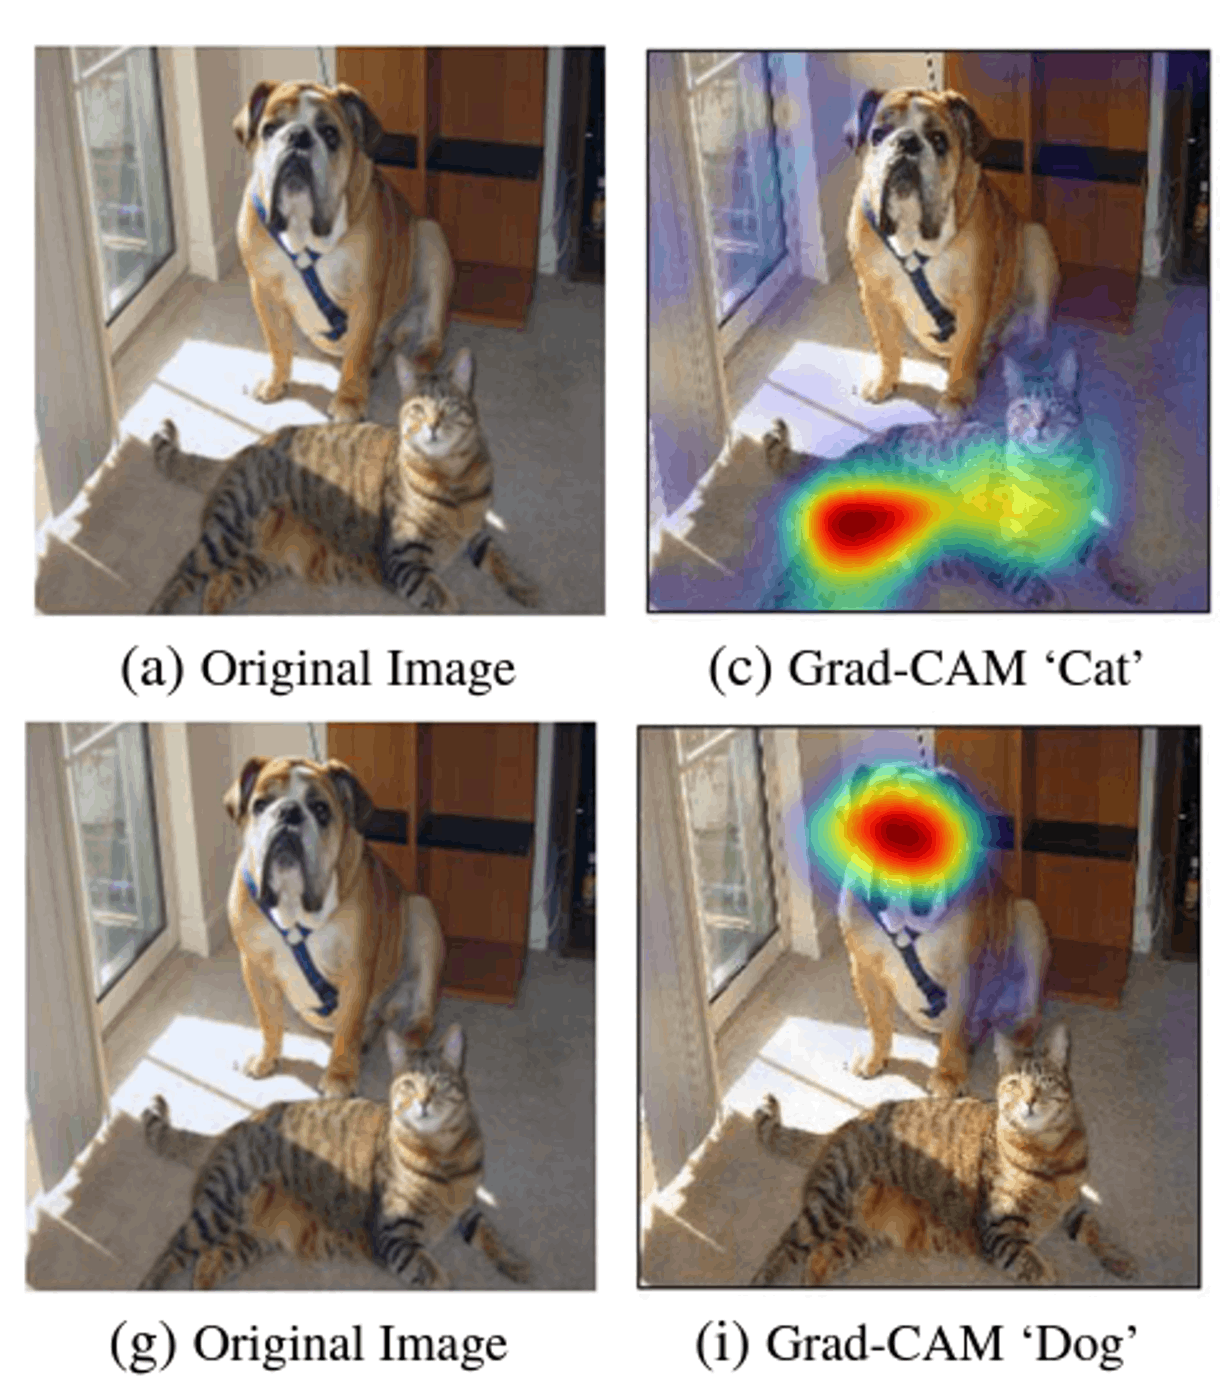
\includegraphics[width=0.5\linewidth]{pictures/explanation/grad_cam_explained.png}
    \caption{画像入力に対するsaliency mapを可視化したもの。1枚の画像に犬と猫が映っているが、犬、猫それぞれのクラス予測に対応する入力箇所が可視化されている。}
    \label{fig:gradcam}
\end{figure}
ある画像に犬が含まれるか、猫が含まれるかを識別する場合は、まずそのカテゴリに属する確率を計算し、そのうえで最大の確率を持つクラスに割り当てるという処理がされる。(Decision theory, 決定理論と呼ばれる)注意すべきは、この画像には、犬に属する確率も猫に属する確率も等しく存在する点である。その上で、Gradcamは、畳み込み層最終の出力の変化が、Sofmax関数に通す前の値にどれだけの変化を起こすのかというものを可視化する。式で言えば、
\begin{equation}
    \alpha_k=\frac{1}{M_k}\sum_i\sum_j{\frac{\partial a^c}{\partial a_{ij}^k}}
\end{equation}
の値を計算し、これらの重みでもって最終層を強調する。
強調すべきは、ニューラルネットにおいては全く同型の写像の機能を持つ関数が学習された場合でも、別々の重みが得られるということである。Bishop\cite{PRML}によれば、これらは同様に良いモデルであるとされる。しかし、今回のような事例では、ある重みのセットよりも好まれる重みのセットが存在する。実機試験においては超音波パルスの形状が機器の性質により扁平になってしまうケースがあり、予測に寄与しない部分にまで同様の重みを割り当てるモデルはロバストな予測に寄与しない。これも結果の章で議論してある。
\section{提案手法}
今、適当な何らかの測定を実行している間、その測定領域における真の値が存在する。これらによって超音波の信号波形が何らかの影響をうけて、測定結果として入手することができる。すなわち、今回の場合は相体積率が潜在変数、測定信号が確率変数として議論を進めるのが適切である。\par
ここで、信号波形から体積率を求めるのと逆の場合、すなわち体積率から信号波形を求める順問題は、比較的容易に解くことができる。固相粒子の個数および一つの粒子の体積、およびその相配置が既知とした場合には、波動方程式に基づく数値的な反復法によって超音波パルスの伝播を再現することができる。よって、数値計算シミュレーションソフトウェアを使用し、ある相体積率及びその相配置に基づく信号波形を生成した。\par
信号波形からそれに対応する相体積率を機械学習で推定する手法の一つには、連続値を推定する回帰モデル、すなわち
\begin{equation}
    p(t | \mathbf{x}, \mathcal{D})
\end{equation}
を推定し、その期待値
\begin{equation}
    \mathbb{E}[t | x ] = \int t p(t |\mathbf{x},\mathcal{D})dt 
\end{equation}
を評価することにより達成できる。よって、その回帰モデルの設計が問題となる。
これらについてだが、設計の要件としては以下のものが挙げられる。\par
・入力信号の現れるピークの位置に関してロバストであること\par
・入力信号は$\mathbb{R}^{1\times W}$の形式を持つ。\par
ここで、信号は極めて長い系列を持ち、全結合型での機械学習モデルの学習にはパラメータ数が発散し計算を行うことが困難である。これらは必ずしも可能ではない。センサーの数並びに配置によっては管内の流動状態を推定するのに十分でない情報しか入手できない場合があるし、ここで用いている仮定が悪い結果を引き起こす可能性についての議論が必要である。以下に、センサーの数および配置に基づく提案手法を示す。\par
\subsection{制約条件}
前述(chapter\ref{experimental settings},page\pageref{experimental settings})のように、本稿で用いた海洋技術安全研究所の実験データは、対向する二つのトランスデューサで円管を挟み、少し離れた位置においてもう一つのトランスデューサを配置するような配置で実験を行った。ここで、超音波パルスを照射したトランスデューサは片側であり対向側は透過波のみを、送信側は反射波および送信した際の信号をそれぞれ記録している。対向側の菅壁内側からの反射波を計測できる場合、透過波の情報は不要であると考え、まずは一つでの学習結果を示す。
実験系では3 kHz でのprf,で5秒間の測定を行っている。すなわち、通算15000回の測定を行っている。これらの測定の度に対応する相体積率が存在するため、1回の測定で相体積率を推定する機械学習モデルを訓練し、時間平均をとる必要がある。

\subsection{アルゴリズム}
前節のような制約・要請を解決する手法として、以下のようなアルゴリズムを提案する。すなわち信号波形を縦1pixelの画像とみなし、CNNやVison Transformerといったスパースな画像学習を行うこととする。
ここで、このような問題設定は極めて異例なものであることに注意が必要である。画像処理分野において、一般的な機械学習の応用としてはあくまで分類的な用法が主流となっているからである。例えば、\cite{Bishop:DeepLearning24}を参照するに、現在広く用いられる画像分野における機械学習の応用には人物検出、顔検出、顔認証、物体認識・識別、音声認識などがあるが、これらはすべて分類タスクである。なぜなら、これらはすべてデータが与えられたときに、そのデータ自身が所定のカテゴリに属する確率を計算するモデルにほかならないからである。\par
確かに、画像から回帰を行っている機械学習モデルは存在する。例えば、R-CNN\cite{girshick2014rich}などは、画像に含まれるObjectのカテゴリを決定すると同時に、その画像のどこにその物体が存在しているのかを決定する。これらの学習は、物体が属するカテゴリの確率を計算する分類モデル並びに、物体の存在するピクセルを目標値とした回帰モデル二者の訓練を同時に行うことによって達成される。ここでは詳細に立ち入らない。注意すべきは、これらの学習は、それらを行う人間の脳の働きを模倣したものということだ。人間の情報処理システムは複雑だが、人間ならば実現可能であるという事実があるからこそ、それを正しく予測する関係性が存在し、それを機械学習で抽出する研究に正当性が生まれる。一方、例えばいくつか人の顔から年齢を予想する研究があるが、\cite{sheoran2020age},\cite{guo2008probabilistic}どれもMAEで85\%~90\% 程度の精度にとどまっている。この理由の一つに、表面的に表れる年の取り方は必ずしも一定ではなく、健康的な人は若く見えるし、不健康な人は老いて見えるというものがある。ゆえに、年の取り方を定義する場合、健康的な人間だけを集めた人間のみを対象とするか、全体的に考慮するかはさらに議論の必要があると\cite{guo2008probabilistic}は述べている。\par
一方で、今回の場合においては、センサーでの値の系列から管内流体の複雑系に含まれる潜在変数の値を推定する回帰モデルを設計する問題である。ここで、機械学習は瞬時の体積率を推定する
\begin{equation}
    \mathbf{x}_n \in \mathbb{R}^{1\times W\times C} \stackrel{f(x,w)}{\to} y_n \in \mathbb{R}^1
\end{equation}
の関数として利用され、通時的な量は
\begin{equation}
    \hat y = \frac{1}{N}\sum_n^N y_n
\end{equation}
によって推定される。
ここで、平均および分散を取得し、エラーバーも取得することができる。平均値においては比較的良好な一致が見られたが、分散が非常に大きくなってしまうという結果が得られた。この問題は、トランスデューサの数を増やし、チャネル数$C$を増やすことによって解決できる可能性がある。その際、センサは対向ではなく垂直に配置した場合には、管内の状態についてより多くの情報を得ることができるため相配置の同定に役立つことが予想される。
\chapter{数値計算結果}
実際の数値計算による結果と、その概要を示す。目安として、研究室の計算環境であるNvidia RTX 4090を利用した場合には、1データあたりおよそ4時間を要した。前節での物性値をもとにして数値計算を行った。
\section{液相のみ}
まず、液相のみのシミュレーションが妥当かどうかを実機をもとに検証する。
\begin{figure}[h]
    \centering
    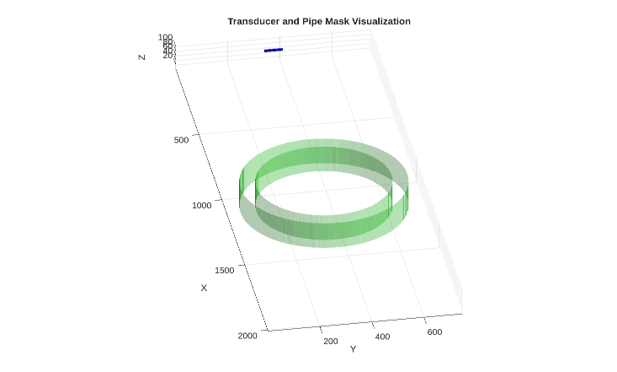
\includegraphics[width=0.5\linewidth]{pictures/results/liquid_only.png}
    \caption{数値計算の計算系の模式図。緑色のものがパイプを模しており、周りを水で満たしているものとする。}
    \label{fig:placeholder}
\end{figure}出力された結果は以下のようなものであった。
\begin{figure}[h]
    \centering
    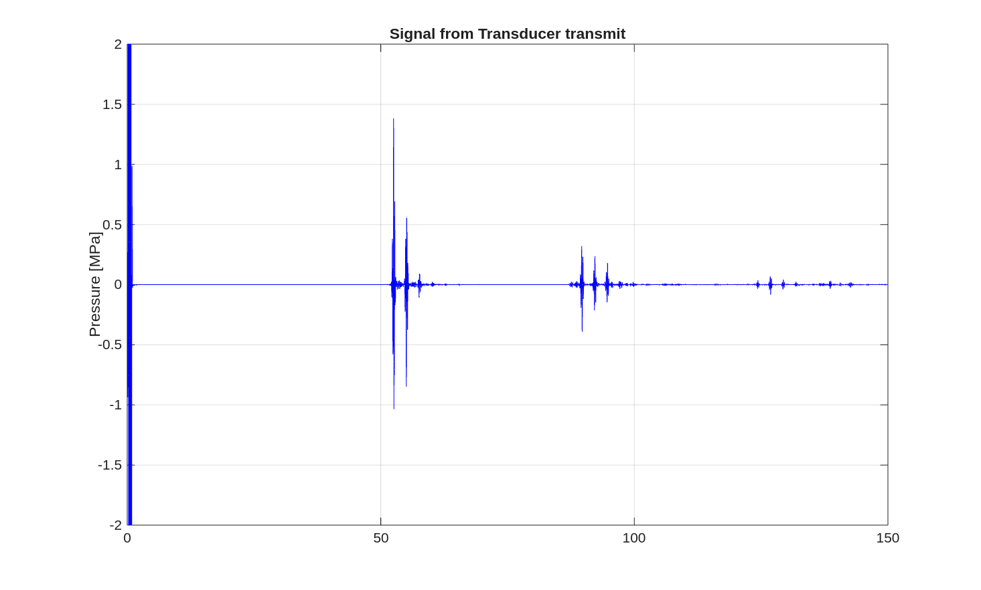
\includegraphics[width=0.5\linewidth]{pictures/results/liquid_only_signal.png}
    \caption{液相のみの場合の信号波形}
    \label{fig:liquid_only}
\end{figure}
液相のみの条件に関しては実際に実験されており、以下のような結果が存在する。一つのデータを示す。
これらの信号波形について、より詳細な解析を行った。
\subsection{超音波厚さ測定}
シミュレーション生成の信号のうち、管壁からのものを詳細に解析する。信号に対してはヒルベルト変換により検波処理を行っており、包絡線を取得してある。このとき、以下の結果が得られる。
\begin{figure}[h]
    \centering
    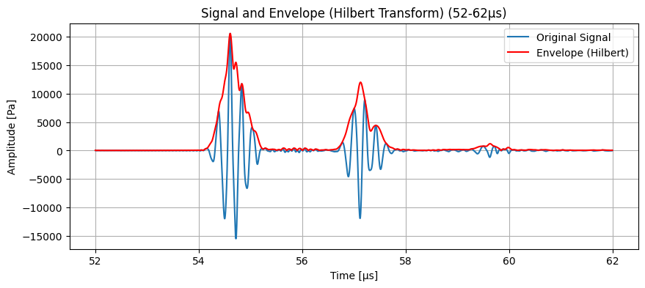
\includegraphics[width=0.5\linewidth]{pictures/results/pipe_refrection_sim.png}
    \caption{Caption}
    \label{fig:placeholder}
\end{figure}
\begin{figure}
    \centering
    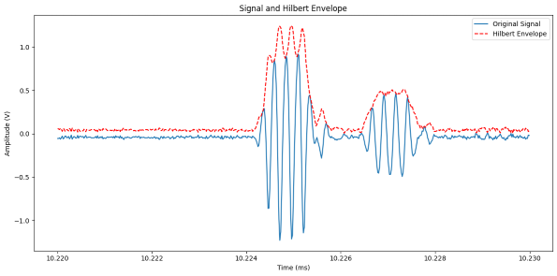
\includegraphics[width=0.5\linewidth]{pictures/results/pipe_refrection_real.png}
    \caption{Caption}
    \label{fig:placeholder}
\end{figure}
これらを比較すると、定性的にはシミュレーション側では山のような形になっており、4回繰り返した信号波形のピークが見えにくい一方で、実機実験の方では先がつぶれたような形状をしていることがわかる。
これらのピークの間の時間差を取得することによって、材質がわかればその厚さが、厚さがわかれば媒体中の音速並びに材質が決定できる。
時刻0を、超音波を照射したタイミングとする。この際、\cite{塩ビ2021}を含む数々の資料でパイプの材質は塩化ビニルだと報告されており、\url{https://ims.evidentscientific.com/}によれば$2395\ \mathrm{m/s}$の伝播速度を持つ。一方で、実測データのピークを詳細に図ると往復で$2.15 \pm 0.019\ \mathrm{\mu s}$の時間差を持つ。これらから算出される厚さは$2.58\ \mathrm{mm}$となるが、事前に報告されていた値である3㎜と合わない。一方で、厚さを$3\ \mathrm{mm}$と仮定した場合の音速は$2790\ \mathrm{m/s}$となり、対応するパイプの材質は「アクリル」となる。\par
今回は情報が不足しているため、材質をアクリルだとみなし音速の値としては$2790\ \mathrm{m/s}$を採用した。
\subsection{フーリエ解析}
次に、この領域に対してフーリエ解析を実行した。まず、実機データのパイプ部分に対する周波数成分を解析する。
\begin{figure}[h]
    \centering
    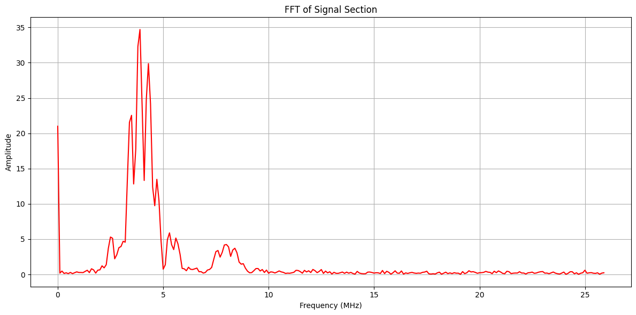
\includegraphics[width=0.5\linewidth]{pictures/explanation/Fourier_analysis_real.png}
    \caption{Caption}
    \label{fig:placeholder}
\end{figure}
これらから、定性的には$4,8\ \mathrm{MHz}$の地点にピークがみられる。使用しているものとちょうど倍の周波数成分がみられるが、これらは倍音(second harmonic)と呼ばれる。\par
次に、数値計算によって生成した信号に対するフーリエ変換を行った結果を示す。以下は$CFL=0.03$で行ったものである。
\begin{figure}[h]
    \centering
    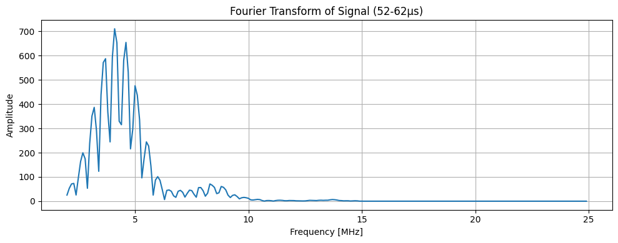
\includegraphics[width=0.5\linewidth]{pictures/explanation/fourier_analysis_sim_0.03.png}
    \caption{CFL=0.03に対する信号波形のフーリエ解析結果。実機と同じ4,8にピークがみられる。}
    \label{fig:placeholder}
\end{figure}
次に、$CFL=0.01$で行った結果を示す。
\begin{figure}[h]
    \centering
    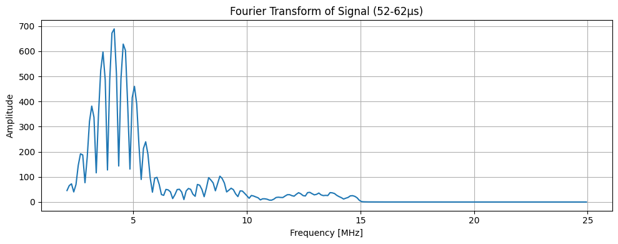
\includegraphics[width=0.5\linewidth]{pictures/explanation/Fourier_analysis_sim_0.01.png}
    \caption{CFL=0.01に対する信号波形のフーリエ解析結果。実機にはない12の成分を持っている。}
    \label{fig:placeholder}
\end{figure}
これらから、周波数空間の観点から、CFLの値としては0.03が好ましいとした。一方で、これらは計算の成立条件を満たしている(\ref{appendix})ので、以下すべてのシミュレーションはこの値のもと行った。
\section{固液二層}
3次元シミュレーションによって計測信号波形を生成した。これらは、機械学習用に使用するものである。基本的に機械学習用データは多いほうが望ましいが、多数は不可能であった。故に100ほどのデータを生成し、それによって訓練を行った。その結果を以下に示す。
\begin{figure}[h]
    \centering
    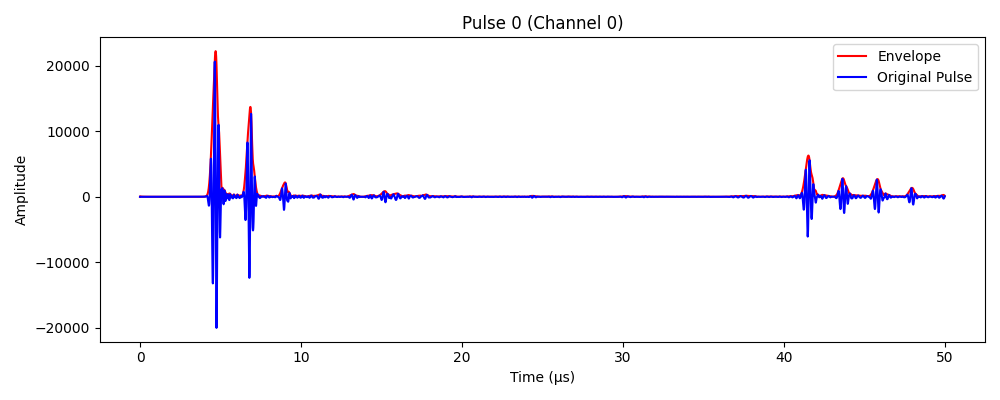
\includegraphics[width=0.5\linewidth]{pictures/results/solid_liquid7_processed_0pulse.png}
    \caption{固相粒子を含めた場合の信号波形}
    \label{fig:solid_liquid}
\end{figure}

\subsection{フーリエ解析}
これらの信号をフーリエ解析することによって、いくつかの有用な特徴を取得できる。現在、測定には4MHzの超音波パルスのみを用いているので、周波数領域においては4MHz付近と、その整数倍のところにピークがみられることが期待される。

これら信号波形は、圧力振幅の形式で記録される。ゆえにその変換を行う。実機とは異なり、パルスは一回のみであり、かつその最大値も数MHzとなることもある。ゆえに、すべての信号の値をその測定範囲内での最大値で除算する操作を行った。これにより、最大値が1であるような信号波形として取得することができる。これをmin-max scalingと呼ぶ。さらに
\chapter{学習結果および予測性能}
回帰モデルをMSE(Mean square error、平均二乗誤差)によって訓練し、その予測精度を評価する。評価に関しては、回帰で一般に用いられるRMSE(Root mean Square error), MAE(Mean Absolute error)を用いた。
\section{固液二層流}
以下は、その予測精度を評価したグラフである。ガラスビーズを固相として用いた場合、石を固相として用いた場合の固相体積率が色分けされてプロットしてある。
\begin{figure}[b]
    \centering
    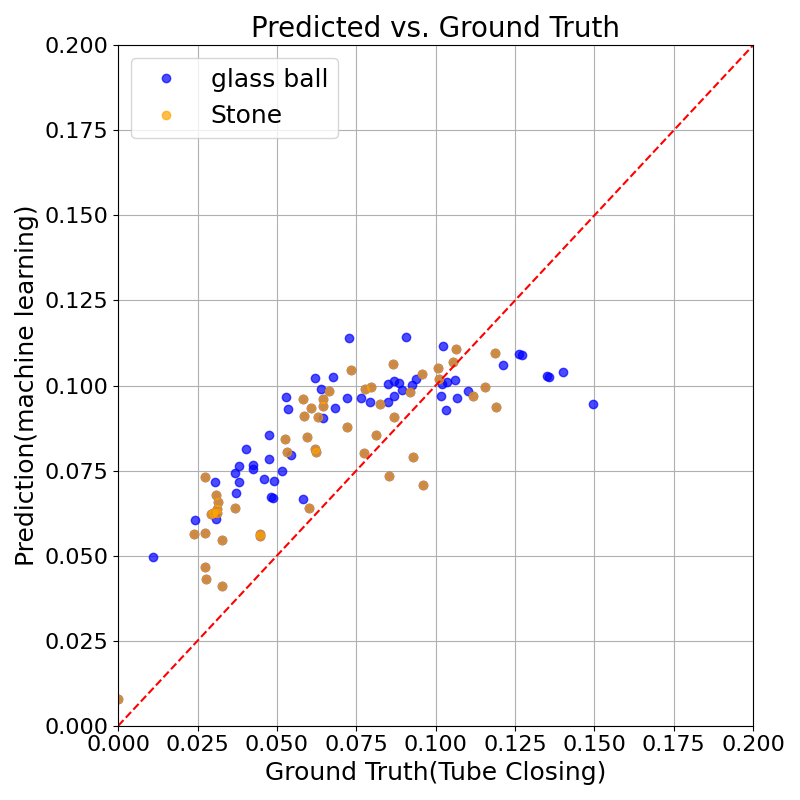
\includegraphics[width=0.4\linewidth]{pictures/results/predicted_vs_ground_truth_noerrorbars.png}
    \caption{縦軸が予測値を、横軸が実測値を示す。ゆえに、点群がy=xに近ければ近いほど精度が高いと判断される。}
    \label{fig:placeholder}
\end{figure}

\newpage
\subsection{課題}
これらテストデータに対する偏りとして、相体積率の最大値が0.15(正確には、2024年データにおいて0.149)というものがあげられる。ゆえに、0から0.15までの値をランダムに予測したり、適当な一次関数からのサンプルでもRMSEの率はそれほど高くはならない。このような議論を行う上では統計検定が必要である。平均すればある程度良い予測結果が得られる一方で、いくつかの欠点がある。まず一つに、機械学習の際、訓練データとテストデータ(実機)の評価が大きくずれる事象が数多く見られた。定性的に一定の類似性はみられるとはいえ、シミュレーションと実機ではデータにあまりに多くの差異がある可能性がある。\par
\begin{figure}[hbp]
    \centering
    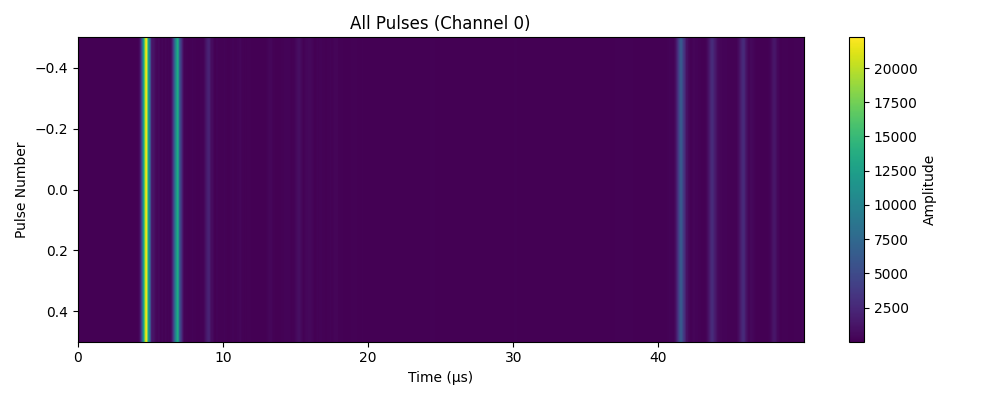
\includegraphics[width=0.5\linewidth]{pictures/explanation/solid_liquid7_processed_0img.png}
    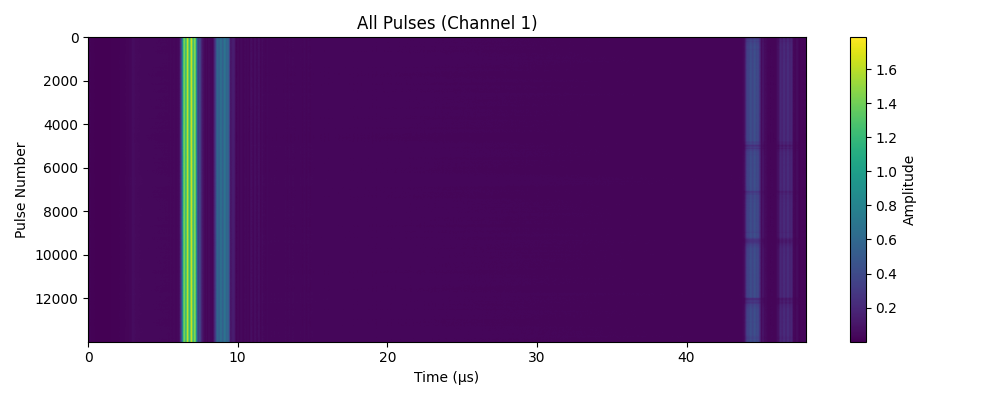
\includegraphics[width=0.5\linewidth]{pictures/explanation/P20240726-1600_processed_1img.png}
    \caption{シミュレーションと実機試験のデータの比較。両者ともに超音波画像法\ref{ultraimage}によって画像化してある。}
    \label{fig:noerrorbar}
\end{figure}
この二つの画像は、そのサンプルである。超音波パルスの幅や、多重反射が明瞭に確認できる回数などに違いが見て取れる。それでも一定の精度を得られたのは、情報処理のメカニズムにおいて、学習の過程でたまたま十分にロバストで実機データを処理するのにも使用可能な局所最適解・パターンを発見したからである可能性が高い。事実、学習率をさげて訓練を行った場合には、訓練データに対してよい精度を示しかつ安定的な学習を行った一方で実機データの値を適切に予測することができなくなった。
だが、それよりも重要なのは、予測に際し分散が非常に大きいということである。上記のグラフは平均値のみをプロットしたが、時間平均を計算する過程で評価できる分散の値も同時にプロットすると
\begin{figure}[b]
    \centering
    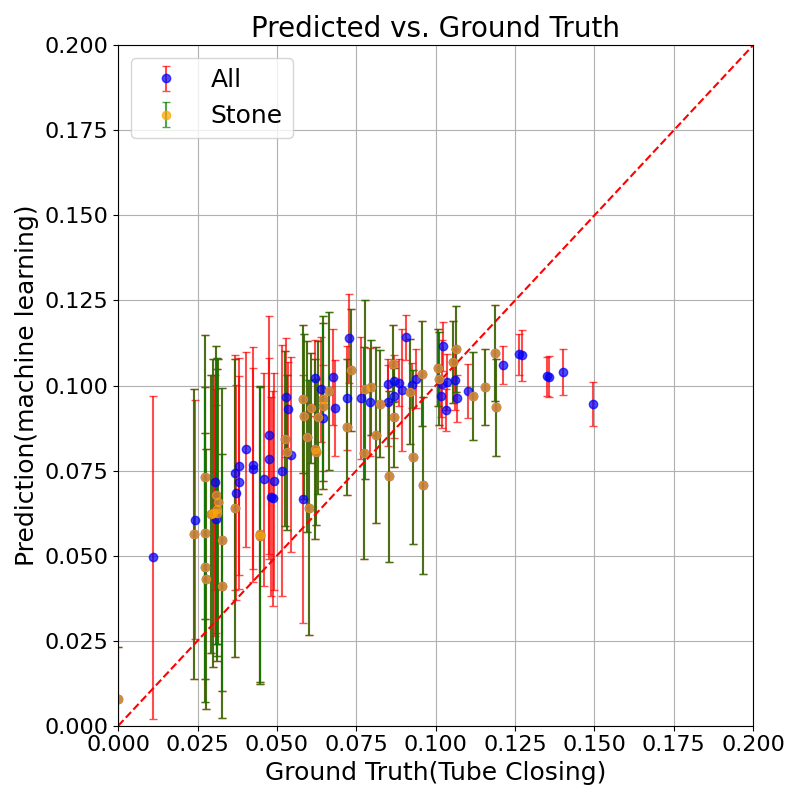
\includegraphics[width=0.5\linewidth]{pictures/explanation/predicted_vs_ground_truth_2.png}
    \caption{Caption}
    \label{fig:errorbars}
\end{figure}
のように、著しくError barが大きく表示されてしまうという問題点がある。これらへの考察として、トランスデューサの数が少ないからというものが挙げられる。機械学習とは統計的なパターン認識技術にすぎないので、予測とは尤もらしい予測とそれに付随する分散によって評価されるからであると考えられる。\par
一方で、実はこれら推定値はリアルタイムにおける相体積率を正しく推定しているという主張もある。実験では5秒間の測定を行っており、3 kHz回の測定の間に真の物理量は明らかに変動しうる。しかし、今回の場合算出したのは平均および分散、標準偏差である。
\subsection{問題解決の提案}
より信頼性の高いモデルを構築しようとした場合に重要なのは、ハイスピードカメラで計測した画像とシミュレーションの予測値を比較することだろう。
\chapter{結論}
\backmatter
\chapter{謝辞}
\bibliographystyle{junsrt}
\bibliography{reference}
\appendix\label{appendix}

\chapter{開発環境と実装・保全}
データ解析を行う上で実装したコードは適切に管理する必要がある。知っておくべき技術は以下の3つである。\par
・Git\par
・Python\par
・Pytorch\par
\section{コード管理}
特に我々チームの研究においてはなぜかプログラミングが当然できるものとして扱われがちなので、最初本当に戸惑うことが多いと思う。どうすればプログラムを実行できるのか、なぜか動かないのだがどうすればいいのかと困る後輩に対し先輩が時間をとって教えるというのも重要なプロセスの一つではあるのだが、無駄が多い。  
そこで、できる限りその作業を書面に残しマニュアル化することによって、本質的な指導に専念できるようになるという体制を構築することを目的とした。その観点から最もコード管理に適したサービスとしてGitHubを採用した。ソフト開発の現場では広く用いられるこのサービスだが、機械学習を導入したいという段階の分野においてはまだまだ知名度が低い。具体的なコマンドに関しては、私のページのReadme.mdに記載しているのでそちらを参照されたい。何も考えずコマンドを打ちこむだけで再現が可能になるという体制を構築した。深い知識を必要とせず動かせるということを第一に考えた。また理解できる内容が増えるほど自由に改造できるようになるという利点がある。
\section{パラメータ管理}
機械学習で最も肝要なのは再現性である。説明してもよくわからないとか言われることも多い上、基本統計ベースの予測なので究極的な理由付けは困難であることが多い。やはり機械学習を用いる一番の理由はその精度にあるので、たまたま評価の際によいグラフや数値が出たとしても、それをなくしてしまったらどうしようもない。あるデータセットで学習して、良い結果が出たとしても、その時のコードを保存するのを忘れてしまったり、モデルを上書きしてしまったり、ハイパーパラメータの設定やアーキテクチャを忘れてしまって、再現できなくなることが非常に多い。モデルに関してはGitで管理するならば問題ないと思うが、Epoch数やハイパーパラメータの管理、そして最も肝要なモデルの保存はしっかりやっておかないとすぐに紛失してしまう。\par
そのような問題に対処し、うまく管理をしてくれるツールとして、hydraというものが挙げられる。Facebook社によって開発されたこのパッケージは、訓練スクリプトが実行された際にその日付と時刻の名前を持つディレクトリを作成し、変数としてそれを格納できる。例えば、2025年10月10日17時10分30秒に訓練スクリプト`train.py`を実行した場合、特定のディレクトリの配下に"2025-10-10/17-10-30"という名前のフォルダを作成し、そこに、ある特定のルールをもってして学習履歴とその際の設定ファイル、saliency mapなどのログや、機械学習のモデルの重みを保存する。これをロードすることにより、いつでもモデルをロードして、予測につかうことができるようになるのだ。これも、重要なのでぜひgithubのページを確認してほしい。\par
他にも、デプロイまでを一連の操作で自動化してくれるmlflow,ハイパーパラメータを探索してくれるhydraなどいろいろなものがあるが、実装には至っていない。また可能ならば、データも保存しておくのが望ましいだろう。
\section{データ管理}
機械学習では、データのバージョン管理も同様に重要である。データセットの中に不適切なものがあった場合には除外する必要があるし、そういった処理がなされていないものを使用してしまうこともある。その意味で、何かの機械学習モデルを作成しようと思った場合には、やはりオンラインストレージを利用した管理を行うことが望ましい。オンラインでデータセットを監視・管理することによってデータベースを構築し、そのディレクトリ構成や要約をドキュメントとして権威化・ルール化する。そのうえで、そのルールを共有し、データローダを構築したり、ノイズ除去などの前処理をするパイプラインを構築すると良いだろう。そこでデータセットのバージョン管理がなされれれば、実行ログと合わせて完全な再現と調査、改善が可能になる。重要なのは、このあたりの手続きを明文化し書類に起こすことである。「推論」に至っては完璧に再現できるので、機械学習済モデルが提案されたが、良いモデルを得るのは一般に難しい。誤った方向に学習が進んでしまうこともあるが、その理由は学習を開始した際の高次元での誤差関数の初期値付近の表面が不安定だからということが考えられる。そのような場合での証拠を残すために、学習履歴はデータのバージョンまできっちり残しておくのが重要である。しかし、そのような体制にはセキュリティの問題が大きく絡んでくるので実現が難しいことも十分考えられる。この環境に関しては、研究室の方針に大きく左右されると思われるので、データの価値を鑑みながら進めることが望ましい。\par
そのような体制が効果的である場合として、以下のような事例が考えられる。本研究は3台のワークステーションで行われた。rtx4090が一台積んであるもの、gtx1080が3台積んであるもの、A4000が2台ついてあるものとなる。これらが同時に高い稼働率を持っていることが望ましいが、例えばどのデータセットをロードするのかが問題となる。今回は暫定的にそれぞれに安価な外付けハードディスクドライブを取り付けて、そこにデータをダウンロードして変換、訓練及び評価に利用したが、データに何らかの問題が生じた場合に、これら3台のPCに手作業で同じ操作を施す必要があった。オンライン上に最新のものが構築されていた場合には、そこからバージョン履歴とともにデータセットをダウンロードしておくスクリプトをgitで管理しておけば、コマンドひとつで同期できるだろう。\par
余談だが、ローカルドライブを同期できるサービスは、筆者の知る限り存在しない。同期させるのであればオンラインにそのコピーを保存する必要があるだろうし、意味がないからだと考えられる。課金してGoogleDriveやAWSなどを用いたほうがいいだろうし、実際の多くの企業はそうしている。個人用のドライブでは、上限が15GB程度でとてもではないが不足する。NASも使用していたが、古かったためか頻繁にクラッシュする事態に遭遇した。また、Droboは公式でWindowsにのみ対応しており、Linuxでドライブを認識させるには自前でパッチを用意する必要があり断念した。余力のある読者諸賢に委ねたい。\par
\section{開発体制}
私よりも一つ上の代での共同研究の体制では、実機データをそのまま機械学習に通すというアプローチが採用されていた。そして、評価指標・目標についての共有は不十分であった。さらに、データがあまりに少ないために、Grad-camの画像をもとに有益な解釈や結論を得るのが難しいという欠点もあった。それらに対し、一般に機械学習の世界での経験則として「前処理に注力することで精度が向上する」というものがあるため、ヒルベルト変換・バンドパスフィルタの適用という思考に至ったと考えられる。\par
これらに対しては、無論データが有限である状況下において最大限の結果を残すという意味で有益ではあるものの、そのデータを増やすことはできないのか、何か別の議論が発生したとして、それらに対処する案をより多角的に検討することが重要である。その観点から、他のグループで使用されている数値計算ソフトウェアを応用してデータを取得するという発想に偶然至り、本研究がなされた。\par
LLMの学習データが不足しているのか、はたまたプロンプトが悪いのかは不明だがGPTモデルが出力する数値計算のコードは間違っていたり、うまく動かないことが極めて多かった。しかし、それでも利用する意義は大きい。以下にその利点を示す。\par
・実機データの改善要素のうち、改善不可能なものと対応可能であるものが一部明確になる。\par
・シミュレーションデータも、一部改良を行うことによって機械学習データセットとして利用できる。\par
Grad-camの画像を確認する際、それが計測機器依存のバリアンスなのか、物理現象として重要な原因なのかを判断することができないという事態が多くみられた。議論の材料さえ不足しており、機械学習のデータセットが不足している状況下においては十分考えられることである。\par
そこで、数値計算ソフトウェアに基づいて計測信号を取得することによって、いくつかの有益な結論を得ることができる。実験系についての論文に基づいて数値計算の前提条件を詳細に設計することにより、支配方程式に基づく理想的な場合の計測データを得ることが可能となるのだ。これにより、シミュレーションに見られる定性的・定量的な特徴と実機測定データにおける同じ特徴量を比較することが可能となり、現象論として原因の究明に寄与することができるのである。さらに、鉛直管内上昇固液二層といった限定的な場合においてはシミュレーションによって生成した信号波形を直接学習し、その予測モデルを利用して比較的良い精度を達成することができた。\par
無論、数値計算結果の章にあるような解析・比較も行い、いくつかの特徴量が統計的に等しいデータセットを学習させてしまっては、事実上実機データを学習させているのと変わらないのではないかという指摘・懸念もありうる。しかし、それでも機器依存のノイズといった再現不可能な量も確かに存在し、それらに対してロバストな学習を行うことができたという意味で、シミュレーションデータセットを学習させる意義はあるだろう。\par
総じて、今後はシミュレーションによってデータを生成し、コードと生成結果を厳密にチェックし、それらをパスした場合のみ学習させるという開発体制が考えられる。そこで、テストは厳密かつ詳細に設計されなければならない。今回も、結果として大きな問題ではないことが示されたものの、いくつかのエラーが示された。今後小さなヒューマンエラーが結果を大きく覆すような事態を引き起こす可能性も十分ある。そこで、実施が望まれるテストを各フェーズに応じて提案する。その内容を以下に示す。\par
\subsection{数値計算}
前述の通り、今回は座標を適切な確率分布からのサンプリングにより生成し、そこに固相を配置し別々な配置パターンでシミュレーションを行うという手続きをとっていると述べた。ここで、今回は残念ながら固相粒子がわずかに重なってしまい、それを発見できなかった。
開発体制としては、まず固相が存在しない単相流のシミュレーションを行い、それらを比較するというアプローチをとった。ここで、信号波形に現れるピークは、超音波パルスの管壁外側の反射、内側の反射、対向側の管壁内側の反射、外側の反射であることは物性値および信号の時間から確認できる。このピークとピークの間の距離を測ることによって、計算系の妥当性を検証してある。\par
次に、ガラス球の半径を実験資料から確認できる値に設定し、1つ、2つ程度真ん中に置いたり、中心から少しずらしたような場所に配置した。これらにより、中心付近にその兆候がみられることを確認した。さらに、ガラス球の座標を変数化し、指定された位置にガラス球が配置されることも確認した。これらのテストにより、ガラス球の座標のセットを入力として数値計算を行う関数が作成されたことが確認されたとみなした。\par
一方で、その座標に関してのテストも行った。前述の通り、$\{x | x\in[-1,1]\},\{y | y\in [-1,1]\},\{z |z \in [0,1]\}$の区間で生成されているが、これらのテストとして$\min_{i,j\in m}d_{ij}, d_{ij}=||r_i-r_j||_2$の値を計算した。これらが適切な閾値よりも上だった場合には、これらは固相として計算系で互いに重ならないことが期待される。シミュレーションに使用した元の値はこれらのテストをパスしていたが、これらを実際の計算系に適用する過程、つまり、[mm]のスケールに合わせて拡大する際の試験を怠っていた。それゆえ、ガラス球がわずかとはいえ重なりあう結果を許してしまった。次回以降、より大規模な開発の際はその試験も追加すべきである。\par
\subsection{信号処理}
基本的にここで扱う処理はフーリエ変換、ヒルベルト変換、信号整形のみである。フーリエ変換のような長い歴史を持つ関数は十分テストされつくしてきたであろうのでテストは不要とした。問題は信号整形である。高次テンソルを扱う都合上、そこからの行列の抽出の際にミスが発生しうるので十分テストされなければならない。\par
特に、実機データにおける処理が肝要である。シミュレーションは実機に合わせればよいが、実機のデータを変換する際は過不足なく情報を抽出せねばならない。これらのファイルに含まれるデータのうち、メタデータを除けばチャンネル数を$C$、信号点数を$L$として$\mathbb{R}^{1\times L \times C}$である。 これらを、測定時に応じて$H$が総測定時間での測定回数と一致するように$\mathbb{R}^{H\times W \times C}$に変換し、測定開始時から無意味と考えられるデータを除外した。この際、チャンネルごとに操作を実施するわけだが、1次元の信号系列から測定時刻を検出し、その時刻を起点として$\mathbb{R}^{W\times H}$に変換したのである。ここで、時刻が正しく検出されているかに関しては、Hのサイズを表示することで確認した。これらが正しく$15000$と表示されていたため実装が正しいとみなした。しかし、解説の通りきわめて自由度の低い柔軟性のない処理であり、よりよい実装が期待される。\par
ヒルベルト変換に関しては、ヒルベルト変換後の信号波形をnp.ndarray配列に格納し、赤でプロットすることによって正しさを検証した。ヒルベルト変換は信号包絡線を取得する目的で行っていたため、実際の信号と重ねてプロットすることによって処理の正しさを視覚的に確認し、正しいとみなした。処理の内容自体に誤りはないと考えられるので、その利用例を注意深く観察し、問題がないと確認した。\subsection{機械学習}
2025年現在、LLMに書かせたコードがエラーなく動くことも多く、簡単なプロンプトを渡すことによってよい結果を出力してくれることは多い。事実、LLMの開発に機械学習を多用しているせいかLLMが出力する機械学習のコードの完成度はほかの分野に比べて高いような感触さえある。しかし、以前として人間がそのコードについて責任を持たねばならず、それを検証する作業が必要である。理論について詳細な理解もなしに開発を進めてしまうと、先入観や思い込みに結果が引きずられてしまう恐れもある。たとえば、「エラーが起きないこと」を目標に開発を行い、コードを理解できる知識なしにGPT駆動の開発を行っていると、テスト用スクリプトの実施を消去する挙動に気づけない。この現象はいくつか報告されており、これを避けるために日々研鑽する必要があるだろう。このあたりを区別するのは一般に難しい。
\chapter{ソフトウェアの仕様、選定について}
ある機能を実現する上で、いくつかのアプローチが考えられるものである。ソフトウェアにおいても例外ではない。ソフトウェアの性質として、計算機上での表現である以上再現性が担保されているというものがあり、教育目的ですべてを自力で実装しなおすという姿勢も十分考えられるだろう。しかし、これらはあまりにも非効率であることが多い。開発には暗黙知が多く、自分で開発したツールは既存のものの劣化版になる可能性が非常に高い。他者が開発したツールは積極的に活用して、できるだけ少ない労力で効率的に目的を達成すべきなのである。その意味で、ライブラリは積極的に活用し、自分が書くコードは最小限にとどめておくほうが無難である。しかし一方で、世には同じ機能をもつが違う名前を持つツールが多数存在する。最終的に実現する内容が同じであれど、ライブラリ毎に内部構造の洗練度に違いがあったり、高速化モジュールが組み込まれていて速度に大きな変化をもたらしたりすることは多い。本付録においては、本論文の目的を達成する上で2025年時点において人気なツールとその性質を簡単に比較し、選定の理由を示す。
\section{数値計算}
使用したコードを\url{https://github.com/apetrasc/kwavesource.git}に示す。\par
引用の通り、kwaveを使用している。実装にはpython,matlabの環境が提供されているが、再現性や研究室のユースケースを考えmatlabを選択した。2025年時点ではAirliftプロジェクト以外にも研究室の多くのメンバーがkwaveを利用して超音波信号波形のシミュレーションを行っていたが、Pythonの環境を利用している者はいなかった。ソフトウェア開発においてはエラーの解決に手間取ることが大変に多いので、近くに似たような事例に遭遇した人がいると大きな助けになることが多い。研究室のメンバーと同じ環境を構築すると利点が大きいので、Matlabベースでの開発を選択した。
\section{信号処理}
処理の全体を\url{https://github.com/apetrasc/psdata2matlab.git}に示す。\par
実際の計測信号は、.psdataと呼ばれる形式で保存されている。この.psdata形式はかなり独自性の強い拡張子であり、2025年時点でpicoscopeという公式のソフトウェア以外は件のデータをロードすることさえできない。さらに公式ソフトウェアに対しても機能を統合し一括で処理を行うこともできない。そこで、何らかの形式に変換する必要があった。\par
ここで、picoscopeにはデータ変換機能が装備されておりその変換後の拡張子にはいくつかの候補があった。従来は.csvに変換し、pandasといったデータ解析ライブラリで読み込み処理するという体制をとっていた。しかし、これでは変換後のファイルサイズが一つあたり7GB程度になるほか、変換に多大な時間を要する問題点があった。確かに、.csvはKaggleといったデータサイエンスコンペティションプラットフォームで広く用いられる拡張子である。しかし、それでもトータルサイズが1GBを超えるのは稀である。今回は一つのファイルが7GBほどのサイズになってしまうので、トータルでは優に1TBを超えてしまう。これでは機械学習のデータを読み込むだけでも多くの時間がかかってしまい、開発に支障をきたす。そこで、バイナリ形式の.matを変換後の拡張子として選択した。これは、名前の通りmatlabで解析もできるほか、pythonの信号処理ライブラリであるscipyにも互換性があるのでデータの変換が容易であるというメリットもある。\par
信号処理を行う際のプログラミング言語、ライブラリの選定も重要である。ここでは、デプロイのしやすさと筆者が慣れているということもあってpythonを選択した。幸い、pythonでは数多くの信号処理ライブラリが存在する。また、近年の機械学習ライブラリは一般にPythonで書かれているので、スクリプトのリファクタリングや処理関数を共有できることができるという点も大きな強みである。信号処理のライブラリとしては、代表的なものにlibrosa, scipy.signal,torchなどがある。このうち、ヒルベルト変換を行うことが必達であるので、その機能が提供されているscipy.signalも利用している。ただ、この問題点としてGPUを使った高速化ができないというものが挙げられる。実機データに対しては15000×5208の信号系列をヒルベルト変換する必要があり、CPUだと決して無視できない時間がかかってしまう。この問題点を解決するため、やむなくtorch環境でのGPUを利用したヒルベルト変換を実装し、利用している。超音波画像法\ref{ultraimage}を利用する上ではヒルベルト変換は不可欠であるため、その実現として以上にあるツールを採用している。\par
拡張子の問題はさらに存在する。Kwaveでは、シミュレーション結果をPicoscopeの変換先である.matの形式で出力することを可能とする。しかし、メタデータはpicoscopeで変換した場合と大きく異なってしまうために同じ関数や機能で信号波形をプロットすることはできない。無論、実機用とシミュレーション用で別々の可視化スクリプトを設計するというアプローチは考えられる。しかし、これでは物理量の厳密な比較の妨げになるだけでなく表示法がずれることが予想され、本質的な違いに注目する妨げにな。故に両者を統一的な.npz形式に変換した。これらは線形代数ライブラリであるNumpyでロードが可能であり、行列の型と統計量をそろえることで区別なくプロットを行うことができると考えた。命名記法としては、(元データの名前).npyが存在した場合に、(元データの名前)\_processed.npzとなるようなファイルを生成するスクリプトを実機・シミュレーションそれぞれで設計して呼び出すという体制をとった。他によい体制を思いついた方がいれば、ぜひ改善してほしい。
関数の命名規則、返り値の型まで詳細にルール化することによって互換性をもたせることができる。
\section{機械学習}
研究に使用したコードを\url{https://github.com/apetrasc/ml_airlift.git}に示す。\par
近年、機械学習の技術が各分野で頻繁に応用され、様々な技術的課題を解決したことが報告されている。その流れを受けて、各分野でも多くの研究がある。しかし、そもそも機械学習を使う必要があるのかについては詳細に議論されなければならない。数理・統計理論、計算機環境の知識を高度に組み合わせる必要のある技術であるため、「なんでも解決してくれる技術」というような誤った理解のまま開発を進めてしまうと高確率で失敗に終わる。近年、生成AIによって実装は以前よりはるかに簡単になったが、依然として万能ではなく、それに気づかないままできるという前提で進めてしまうと技術員が疲弊する結果になりかねない。以下に機械学習の援用が効果的な場合を示す。
\begin{description}
    \item[1.]そもそも、何らかの手段でその一部が可能であるとわかっているとき
    \item[2.]データが存在するとき
    \item[3.]明確な理論を構築するのが難しい時
\end{description}

データが存在しないのにも関わらず機械学習を使用することはできない。故に計算機科学の世界では、データセット生成だけでも論文になりうる。それでも機械学習を用いようとした場合にはデータセットを新たに開発する必要があり、コストが膨大になってしまう。
明確な理論を構築するー
研究目的では、可読性と保守性の観点からFacebookが開発した深層学習ライブラリであるpytorchを用いるのが最も望ましいと考え、本研究においてもこのフレームワークを用いて実装を行った。このフレームワークはAPIが豊富であり、基礎的なMLP(多層パーセプトロン)やCNN(畳み込みニューラルネットワーク)というモデルだけでなく、ベイズ統計の基礎を成すガウス過程や、近頃人気の生成モデルを設計するためのVAE(変分オートエンコーダ)などのモデルを容易に実装できるようになっている。Pytorchによって記述されたコードは人間による解釈が容易であり、かつ環境構築が非常に容易であるという観点から採用を行った。他には、Google社によるTensorflow,かつて世界の先駆けだった日本スタートアップPFN社製のChainerなどがある。これらに関して、Tensorflowは筆者の経験上再現が極めて煩雑であったり、同じコードでも動かないということが頻発するので、推奨しない。実体験をもとに語れば、筆者の留学先ではTensorflowを用いた開発を行っていたのだが、全く同じコードのまま2021年という比較的新しい時期に書かれたのにも関わらず、実行できないという事態に遭遇した。これは、開発者本人によるとサーバー上で環境を設定する際に、当時のモジュールが消失してしまっただけではなく、TensorflowのAPIの変数名と機能が変わってしまったがために起きたことであったようだ。GPTモデルをふんだんに駆使して実行してもうまくいかなかったので、開発者に相談して、深層学習を本でしっかり勉強して一行一行書き直して事なきを得た。他方、Pytorchではそういったことがない。極めて数学的に実装する必要がある以上多少書くのが難しいというデメリットはあるが、機能が途中で大幅に変更されて動かなくなるといったことは筆者の知る限り聞かない。\par
以上の理由により、Pytorchの利用を進める。\cite{torchvstensor}によれば、研究分野においてTensorflowよりもPytorchのほうが4倍多い利用者を持つ。
\chapter{数学的準備}
機械学習は統計的な手法であり、アルゴリズムの設計にもその性能評価にもいくつかの数学的準備を必要とする。ここでは、用いた議論や論拠の補足を行う。
\section{指標}
分類・回帰の性能評価に関する議論を行う。分類モデルに関しては精度・再現率・F値といった数々の指標が良く議論されている一方で、回帰タスクにおいては十分に行われていないようである。ここでは、その性能指標について、今回RMSEをMAEよりも好むかの理由について述べる。\par
そもそも、今回は固相体積率という連続値をとる量を推定する目的で研究が行われてきた。その理由は、構成方程式の精度を検証するためであった。誤差が生じる状況を大きく二分するとすれば、次の二つのケースが考えられる。
\begin{description}
    \item[1.] 全体的に中程度の誤差が出て、大きな誤差を取るものが極めて少ない
    \item[2.] 全体的に小程度の誤差が出て、一部のみ大きな誤差を取るものが存在する。
\end{description}
このうち、精度を検証する目的では全体的な中程度の誤差は、一部の大きな誤差よりも優先される。MAEではその誤差に対して線形な損失を割り当てるのに対し、MSEではその誤差の二乗の損失を割り当てる。それゆえ、L1Loss(MAE)よりもL2Loss(MSE)のほうが望ましい。さらに言えば、ある程度の誤差が許容されるのであればより高次のLossを用いるのさえ望ましい。MAEを利用しない理由はこれである。
\end{document}
